\section{Introduction}
\showtoc

\subsection{Motivation}

\begin{frame}[t]
  \frametitle{Motivation}
  \only<1> {
    \begin{block}{Goal}
      Design an optimal controller to shape the energy dynamics of periodic
      behaviors in mechanical systems without destroying stability.
    \end{block}

    \begin{block}{Considerations}
      \begin{itemize}
      \item Should work on systems with impulse effects
      \item Should be computationally tractable
      \item Should not alter the steady-state periodic behavior
      \item Control law should be guaranteed to exist at least locally
      \end{itemize}
    \end{block}
  }

  \only<2>{
    \begin{block}{Problem}
      Certain controllers induce periodic behaviors \red{but}
      altering gains can change overall trajectory.
    \end{block}
      
    \begin{block}{Question}
      How can we make such controllers more robust without altering the
      steady-state behavior?
    \end{block}

    \begin{block}{Solution}
      Take advantage of the periodic nature of energy to stabilize the energy
      dynamics.
    \end{block}
  }
\end{frame}

\begin{frame}[t]
  \frametitle{Existing Results}
  \begin{block}{Total energy shaping and controlled symmetries}
    \small
    M. W. Spong, J. K. Holm, and D. Lee. {\em Passivity-based control of
      bipedal locomotion}. IEEE T. Robotic. Autom., 14(2), pp.~30--40,
    2007.
  \end{block}
  \begin{block}{Controlled Lagrangians}
    \small
    A. M. Bloch, N. E. Leonard and J.E. Marsden. {\em Controlled Lagrangians
      and the stabilization of mechanical systems I: The first matching
      theorem}. IEEE T. Automat. Contr., 45(12), pp.~2253--2270, 2000.
  \end{block}
  \begin{block}{Rapidly exponentially stabilizing control Lyapunov functions}
    \small
    A. D. Ames, K. Galloway, K. Sreenath, and J. W. Grizzle. {\em Rapidly
    exponentially stabilizing control Lyapunov functions and hybrid zero
    dynamics}. IEEE T. Automat. Contr., 59(4), pp.~876--891, 2014.
  \end{block}
\end{frame}

\newcommand{\fgap}{\vspace{-.8em}}

\begin{frame}[t]
  \frametitle{Passive Dynamic Walking}
  \vspace{-1em}
  \begin{columns}    
    \column{.5\textwidth}
    \begin{figure}
      \centering
      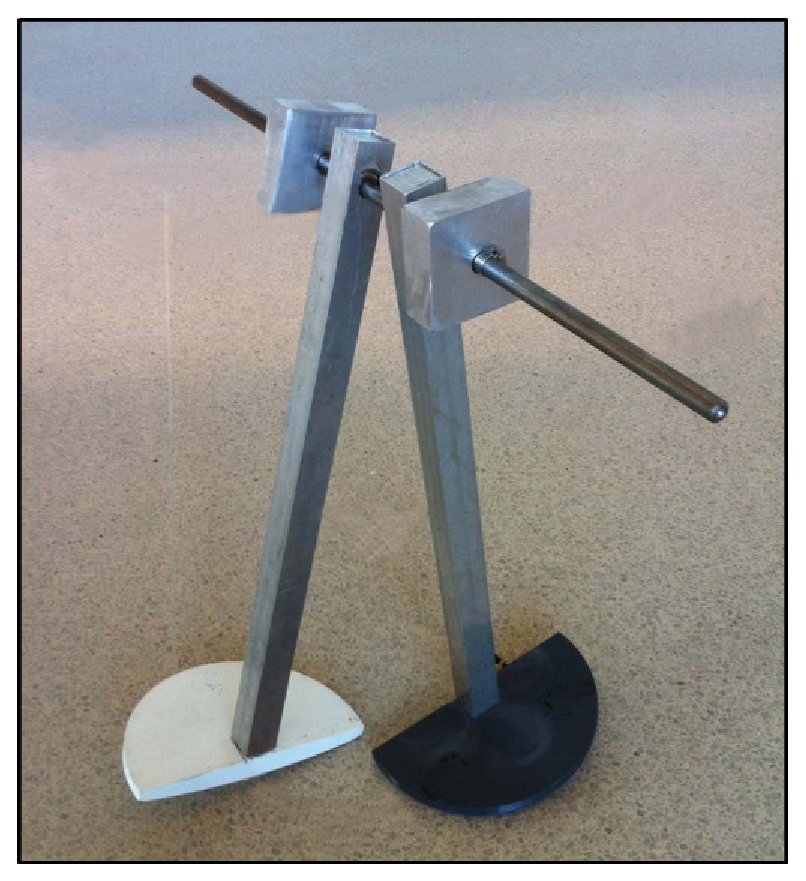
\includegraphics[height=.75\textheight]{compass-gait}
      \fgap
      \caption{Passive compass gait biped}
    \end{figure}
    
    \column{.5\textwidth}
    \begin{figure}
      \centering
      \includegraphics[height=.75\textheight]{bipeds_collins}
      \fgap
      \caption{Passivity-based control}
    \end{figure}
  \end{columns}
\end{frame}

\begin{frame}[t]
  \frametitle{Hybrid Zero Dynamics}
  \vspace{-1em}
  \begin{columns}
    \column{.5\textwidth}
    \begin{figure}
      \centering
      \includegraphics[height=.75\textheight]{bipeds_grizzle}
      \fgap
      \caption{RABBIT -- Grizzle}
    \end{figure}
    
    \column{.5\textwidth}
    \begin{figure}
      \centering
      \includegraphics[height=.75\textheight]{bipeds_ames}
      \fgap
      \caption{AMBER 2 -- Ames}
    \end{figure}
  \end{columns}
\end{frame}
